% Research proposal, Option B (modern two-tone journal style). Build: latexmk -xelatex proposal.tex
\documentclass[11pt,a4paper]{article}

\usepackage[a4paper,margin=2.4cm,headheight=24pt,headsep=12pt]{geometry}
\usepackage{fontspec}
\setmainfont{Times New Roman}
\newfontfamily\headfont{Arial}
\usepackage{microtype}
\usepackage{setspace}
\setstretch{1.15}
\usepackage[table]{xcolor}
\definecolor{accent}{HTML}{7A1F3D}
\definecolor{accentlight}{HTML}{F3E6EA}
\definecolor{warmgrey}{HTML}{6B6B6B}
\definecolor{sidebg}{HTML}{F5F2F0}
\usepackage{titlesec}
\usepackage{booktabs,array,tabularx}
\usepackage{enumitem}
\usepackage{needspace,etoolbox}
\pretocmd{\section}{\needspace{5\baselineskip}}{}{}
\pretocmd{\subsection}{\needspace{3\baselineskip}}{}{}
\usepackage{fancyhdr}
\usepackage{lastpage}
\usepackage{tikz}
\usetikzlibrary{positioning,arrows.meta,calc}
\usepackage{csquotes}
\usepackage[backend=biber,style=numeric,sorting=none,maxbibnames=3,minbibnames=1,giveninits=true,doi=true,url=false,isbn=false]{biblatex}
\addbibresource{../refs.bib}
\usepackage[hidelinks,pdftitle={Segmenting Gliomas When Sequences Are Missing: A Controlled Comparison of Training Strategies for Incomplete Multimodal MRI},pdfauthor={Qarar Hussain}]{hyperref}

\setlist{nosep,leftmargin=1.6em}
\setlength{\parindent}{0pt}\setlength{\emergencystretch}{2em}
\setlength{\parskip}{4pt}
\renewcommand{\arraystretch}{1.15}
\newcommand{\tbp}{\textcolor{accent}{[to be provided]}}

% headings: sans-serif, burgundy
\titleformat{\section}{\headfont\large\bfseries\color{accent}}{\thesection}{0.7em}{}
\titleformat{\subsection}{\headfont\normalsize\bfseries\color{warmgrey}}{\thesubsection}{0.6em}{}
\titlespacing*{\section}{0pt}{12pt}{4pt}
\titlespacing*{\subsection}{0pt}{7pt}{2pt}
\usepackage{caption}
\captionsetup{labelfont={bf,color=accent},font=small,labelsep=period}

% running header / footer
\pagestyle{fancy}
\fancyhf{}
\renewcommand{\headrulewidth}{0.4pt}
\renewcommand{\headrule}{\hbox to\headwidth{\color{accent}\leaders\hrule height \headrulewidth\hfill}}
\fancyhead[L]{\headfont\footnotesize\color{warmgrey} Segmenting Gliomas When Sequences Are Missing}
\fancyhead[R]{\headfont\footnotesize\color{warmgrey} Research Proposal}
\fancyfoot[L]{\headfont\footnotesize\color{warmgrey} Qarar Hussain}
\fancyfoot[R]{\headfont\footnotesize\color{warmgrey} Page \thepage\ of \pageref{LastPage}}
\fancypagestyle{first}{\fancyhf{}\renewcommand{\headrulewidth}{0pt}%
  \fancyfoot[L]{\headfont\footnotesize\color{warmgrey} Qarar Hussain}%
  \fancyfoot[R]{\headfont\footnotesize\color{warmgrey} Page \thepage\ of \pageref{LastPage}}}

\begin{document}
\thispagestyle{first}

% ---------------- Title block with metadata side bar ----------------
\noindent
\begin{minipage}[t]{0.665\linewidth}\vspace{0pt}
  {\headfont\footnotesize\bfseries\color{warmgrey}\MakeUppercase{Research proposal \;|\; Master's thesis}\par}
  \vspace{6pt}
  {\raggedright\hyphenpenalty=10000\headfont\bfseries\fontsize{21}{25}\selectfont\color{accent} Segmenting Gliomas When Sequences Are Missing\par}
  \vspace{6pt}
  {\raggedright\hyphenpenalty=10000\itshape A Controlled Comparison of Training Strategies for Incomplete Multimodal MRI\par}
  \vspace{4pt}
  {\color{accent}\rule{\linewidth}{0.8pt}}\par
  \vspace{2pt}
  {\headfont\small\bfseries\color{accent} Abstract}\par
  \small\setstretch{1.1}\sloppy
  Brain MRI examinations usually contain four sequences (T1, contrast-enhanced T1, T2 and FLAIR) that show different tissue properties. In routine care one or more sequences are often missing, and a segmentation model trained only on complete cases can then fail without warning. This proposal plans a controlled, reproducible study of brain-tumour segmentation under missing modalities. We will train a compact 3D U-Net on the BraTS 2023 glioma data and measure the change in Dice and HD95 for all 15 non-empty modality subsets. We will then compare three strategies on identical subject-level splits: a complete-input model with zero-filled gaps, modality dropout, and modality dropout with explicit presence indicators. Two extensions are optional and depend on time and compute: training with 100, 50, 25 and 10\% of the segmentation masks, with or without self-supervised pretraining, and a cross-release check that will be called external validation only if dataset independence is shown. All hypotheses and the evaluation protocol are fixed before any test result is seen, and the study is sized for a 4~GB GPU. This is a research study, not a clinical tool.
\end{minipage}\hfill
\begin{minipage}[t]{0.29\linewidth}\vspace{0pt}
  \setlength{\fboxsep}{9pt}
  \colorbox{sidebg}{\parbox{\dimexpr\linewidth-2\fboxsep\relax}{\raggedright\headfont\footnotesize\setstretch{1.1}
    {\bfseries\color{accent} Student}\\ Qarar Hussain\\[5pt]
    {\bfseries\color{accent} Roll number}\\ \tbp\\[5pt]
    {\bfseries\color{accent} Supervisor}\\ Kalitin Denis Vladimirovich\\[5pt]
    {\bfseries\color{accent} Program}\\ Data Science, direction 09.04.01 (Master's)\\[5pt]
    {\bfseries\color{accent} University}\\ NUST MISIS, College of IT \& Computer Science, Department of Computer-aided Design and Engineering Design\\[5pt]
    {\bfseries\color{accent} Date}\\ Moscow, 2026\\[5pt]
    {\bfseries\color{accent} Keywords}\\ brain MRI; tumour segmentation; missing modalities; modality dropout; label efficiency; reproducibility}}
\end{minipage}

\vspace{8pt}
\noindent\setlength{\fboxsep}{8pt}\fcolorbox{accent}{accentlight}{\parbox{\dimexpr\linewidth-2\fboxsep-0.8pt\relax}{\small\setstretch{1.1}
  {\headfont\bfseries\color{accent} Key idea.} Missing sequences are common in practice. We will measure, on identical subjects and splits, how much a compact 3D U-Net loses for each of the 15 possible sets of available sequences, and test whether two cheap training changes (modality dropout and presence indicators) recover that loss.}}

% ---------------- 1 ----------------
\section{Introduction and Motivation}
Gliomas are the most common primary brain tumours in adults. To plan treatment, clinicians need to know where the tumour is and which parts are active, swollen or dead tissue. This is done on MRI (magnetic resonance imaging), where each \emph{sequence} (or \emph{modality}) highlights something different: T1 shows anatomy, contrast-enhanced T1 (T1ce) highlights active tumour, T2 shows fluid and swelling (oedema), and FLAIR suppresses free fluid to expose lesions. Drawing the tumour by hand on all four is slow, so automatic segmentation is an active research area with a public benchmark, BraTS \cite{menze2015,bakas2018}.

Most published models assume that all four sequences exist at test time. In practice a sequence may be skipped, corrupted, or never transferred between systems. A model trained on complete cases and fed a blank channel may lose much of its accuracy, and the user is not told. The simple fixes (training only on complete cases, or filling the gap with zeros) are rarely compared fairly with each other. A reliable answer to ``how much do we lose, and what is the cheapest way to lose less?'' is therefore useful.

The project will not diagnose patients or claim clinical safety; it is a reproducible measurement on public research data.

% ---------------- 2 ----------------
\section{Background and Related Work}
\textbf{Data.} BraTS provides multi-institutional glioma MRI with expert segmentations of three nested regions: whole tumour (WT), tumour core (TC) and enhancing tumour (ET) \cite{menze2015,bakas2017,baid2021}. The Medical Segmentation Decathlon (MSD) includes a brain-tumour task built from BraTS-related data \cite{antonelli2022}. Because the two sources may share cases, we will treat them as possibly overlapping (Section~\ref{sec:data}).

\textbf{Segmentation backbones.} The U-Net and its 3D version are the standard encoder--decoder for medical volumes \cite{ronneberger2015,cicek2016}. nnU-Net showed that a well-configured plain U-Net is a very strong baseline across tasks \cite{isensee2021}. We therefore use a compact 3D U-Net and design no new architecture.

\textbf{Missing modalities.} Three groups of methods are known. (i)~\emph{Shared-representation} models encode each modality separately and fuse whatever is present, for example HeMIS \cite{havaei2016}, feature disentanglement with gated fusion \cite{chen2019}, and region-aware fusion \cite{ding2021}. (ii)~\emph{Completion} models try to synthesise the missing sequence while segmenting \cite{dorent2019}. (iii)~\emph{Transformer-based} fusion handles incomplete inputs with attention across modalities \cite{zhang2022}. A cheaper idea, \emph{modality dropout}, randomly hides input channels during training so the network learns not to depend on one of them; it was proposed for multimodal gesture recognition \cite{neverova2016}.

\textbf{Label efficiency.} Self-supervised pretraining learns features from unlabelled volumes before fine-tuning on a few masks \cite{zhou2021,tang2022}. Whether it helps brain-tumour segmentation at low label counts, on top of a compact model, is something we will test, not assume.

\textbf{Gap (working claim, to be confirmed by the literature review).} Many incomplete-modality papers introduce new architectures. We have not yet confirmed how many compare the simple strategies (zero-fill, modality dropout, presence indicators) on identical subject-level splits, over all 15 subsets, with paired statistics, under a small-GPU budget. If the review finds this is already covered, the claim and the contribution will be rewritten.

% ---------------- 3 ----------------
\section{Problem Statement, Research Questions and Hypotheses}
\textbf{Problem.} How reliable is brain-tumour segmentation when one or more MRI modalities are missing, which practical strategy keeps it most reliable, and can unlabelled data reduce the need for expert masks?

The research questions (RQ) and hypotheses (H) in Table~\ref{tab:rq} are written before any experiment. Tests are paired over test subjects, with Holm correction and 95\% bootstrap confidence intervals.

\begin{table}[ht]
\centering\small
\caption{Research questions, hypotheses, outcomes and tests. WT, TC, ET: whole tumour, tumour core, enhancing tumour.}
\label{tab:rq}
\begin{tabularx}{\linewidth}{@{}l>{\raggedright\arraybackslash}X>{\raggedright\arraybackslash}X>{\raggedright\arraybackslash}p{2.9cm}@{}}
\toprule
\rowcolor{accentlight}\textbf{RQ} & \textbf{Question and hypothesis} & \textbf{Outcome} & \textbf{Test} \\
\midrule
RQ1 & How much does segmentation quality fall when modalities are missing? \newline \emph{H1: for every region, mean Dice with any missing modality is lower than with all four; the size of the fall depends on which modality is missing.} & Dice and HD95 per region and per subset (15 subsets); fall relative to complete input & Paired Wilcoxon signed-rank, Holm over subsets \\
RQ2 & Which strategy is most robust? \newline \emph{H2: modality dropout raises mean Dice over the 14 incomplete subsets compared with the zero-filled complete-input model; adding presence indicators raises it further (exploratory).} & Mean Dice over incomplete subsets; cost on complete input & Paired Wilcoxon, bootstrap CI \\
RQ3 & Do fewer masks hurt, and does self-supervised pretraining help? \newline \emph{H3: with 25\% or fewer of the masks, a pretrained encoder gives higher Dice than training from scratch.} (optional) & Dice at 100, 50, 25, 10\% of masks & Paired over subjects, across seeds \\
RQ4 & Do conclusions hold on a different data release? \newline \emph{H4: Dice is lower on a different release than on the internal test set.} (optional, descriptive unless independence is shown) & Dice and HD95 on the other release & Bootstrap CI; no test if overlap exists \\
\bottomrule
\end{tabularx}
\end{table}

% ---------------- 4 ----------------
\section{Objectives}
\begin{enumerate}
  \item \textbf{Build} a tested data pipeline that loads, maps and visualises images and masks from MSD and BraTS 2023, with explicit label and channel-order mapping per dataset (RQ1--RQ4).
  \item \textbf{Train} a compact 3D U-Net baseline on complete inputs and report its Dice and HD95 for WT, TC and ET (RQ1).
  \item \textbf{Measure} the performance of that baseline on all 15 non-empty modality subsets (RQ1).
  \item \textbf{Compare} zero-fill, modality dropout, and modality dropout with presence indicators on identical splits and subjects (RQ2).
  \item \textbf{Test}, if time and compute allow, the effect of 100, 50, 25 and 10\% of masks, with and without self-supervised pretraining, and a cross-release check (RQ3, RQ4).
  \item \textbf{Release} reproducible code, configurations, split files and a data card, without any medical images (all RQs).
\end{enumerate}

% ---------------- 5 ----------------
\section{Data}\label{sec:data}
\textbf{BraTS 2023 GLI (main dataset).} Official source: the BraTS 2023 glioma challenge on Synapse. Each case has four co-registered modalities and expert labels. The training archive (about 1,250 cases expected; the exact number is recorded by the data audit), the validation archive and a 2023-to-2017 case-identifier mapping file are being downloaded. \emph{Public validation masks must not be assumed}; if they are absent, that archive is not used for scoring. Labels will be taken from the challenge specification and checked by a test, not assumed from other years.

\textbf{MSD Task01 Brain Tumour (development).} Official source: the Medical Segmentation Decathlon. Used first for building and debugging the pipeline. Case count, modality order and label meaning will be read from the downloaded files and documentation and recorded in the data card.

\textbf{Overlap.} MSD and BraTS releases may share source cases. The identifier mapping and documentation will be checked before any cross-release result is reported; without shown independence the result is called ``cross-release evaluation'' with a stated limitation, never ``external validation''.

\textbf{Terms and ethics.} Both datasets will be used only under their published licences and data-use terms, which are recorded in the data card before any result is shared; if the university requires ethics review for public research data, it will be completed first. No images or volumes are committed to the repository.

\textbf{Splits.} Splits are made at \emph{subject} level (never slice or patch) with a fixed seed, saved as files of subject identifiers, and checked by a leakage test. Proposed ratio 70/15/15 for train/validation/test. The test set is used once, after the protocol and all choices are frozen.

% ---------------- 6 ----------------
\section{Methodology}
Figure~\ref{fig:pipeline} shows the pipeline. Every number in the thesis will come from a seeded script with a logged configuration.

\begin{figure}[ht]
\centering
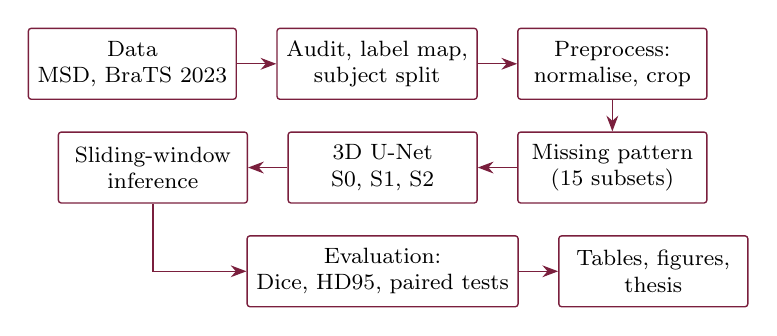
\begin{tikzpicture}[
  node distance=4mm and 5mm,
  box/.style={draw=accent, rounded corners=1pt, minimum height=9mm, minimum width=24mm, align=center, font=\footnotesize, line width=0.5pt},
  arr/.style={-{Stealth[length=2mm]}, line width=0.5pt, color=accent}]
  \node[box] (d) {Data\\MSD, BraTS 2023};
  \node[box, right=of d] (s) {Audit, label map,\\subject split};
  \node[box, right=of s] (p) {Preprocess:\\normalise, crop};
  \node[box, below=of p] (m) {Missing pattern\\(15 subsets)};
  \node[box, left=of m] (t) {3D U-Net\\S0, S1, S2};
  \node[box, left=of t] (i) {Sliding-window\\inference};
  \node[box, below=of t] (e) {Evaluation:\\Dice, HD95, paired tests};
  \node[box, right=of e] (r) {Tables, figures,\\thesis};
  \draw[arr] (d)--(s); \draw[arr] (s)--(p); \draw[arr] (p)--(m);
  \draw[arr] (m)--(t); \draw[arr] (t)--(i); \draw[arr] (i) |- (e);
  \draw[arr] (e)--(r);
\end{tikzpicture}
\caption{Method pipeline. S0: complete-input model with zero-filled gaps; S1: modality dropout; S2: modality dropout with presence indicators. The missing pattern is applied to the input channels of the same test subjects for every strategy.}
\label{fig:pipeline}
\end{figure}

\subsection{Preprocessing}
Images and masks are loaded with NiBabel and MONAI \cite{cardoso2022}. We check orientation, spacing, shapes and image--mask alignment on a few cases before any training. Intensities are normalised inside the brain (z-score per modality), volumes are cropped to the foreground, and training uses random 3D patches. Discrete masks are never interpolated with a continuous filter. Augmentation is applied to training cases only, with the same spatial transform on image and mask.

\subsection{Model and training}
A compact 3D U-Net (about 16--32 base channels, set by the memory test) with Dice plus cross-entropy loss, mixed precision, small patches and batch size one, with gradient accumulation if needed. Patch size, learning rate and schedule are tuned on validation data only and recorded.

\subsection{Compared strategies and ablations}
\textbf{S0 (reference).} Trained on complete inputs; at test time a missing channel is set to zero, which equals the mean after z-scoring. \textbf{S1 (modality dropout).} During training each case draws a random non-empty subset of modalities; missing channels are zero-filled \cite{neverova2016}. \textbf{S2 (dropout plus presence indicators).} As S1, plus four binary input maps that tell the network which modalities exist. Ablations: dropout probability, and cost on complete input. Optional: S0 and S2 trained on 100, 50, 25 and 10\% of masks, from scratch or from a self-supervised encoder \cite{zhou2021,tang2022}. Heavier architectures \cite{havaei2016,zhang2022} are discussed, not re-implemented.

\subsection{Evaluation protocol}
The protocol in Table~\ref{tab:eval} is fixed before test results are seen. Metric choice follows the segmentation-metrics literature \cite{taha2015,maierhein2024}. Voxel accuracy is not used, because background dominates.

\begin{table}[ht]
\centering\small
\caption{Evaluation protocol. All metrics are computed per subject and per region (WT, TC, ET) and per modality subset.}
\label{tab:eval}
\begin{tabularx}{\linewidth}{@{}>{\raggedright\arraybackslash}p{2.3cm}>{\raggedright\arraybackslash}X>{\raggedright\arraybackslash}X>{\raggedright\arraybackslash}p{2.6cm}@{}}
\toprule
\rowcolor{accentlight}\textbf{Metric} & \textbf{How computed} & \textbf{Empty-case rule} & \textbf{Test / RQ} \\
\midrule
Dice & Overlap of prediction and reference & Both empty: 1; only one empty: 0 & Paired Wilcoxon, Holm (RQ1--4) \\
HD95 & 95th percentile surface distance in mm using voxel spacing & Undefined if either is empty: counted and reported, not imputed & Same \\
Sensitivity, precision & Voxel recall and precision of the region & Same rule as Dice & Descriptive \\
Thresholds & Class decision (argmax or 0.5 per region) and checkpoint chosen by mean validation Dice over all 15 subsets & Validation data only & Frozen before test \\
Uncertainty of results & 95\% bootstrap CI over subjects (10{,}000 resamples); $\geq3$ seeds if compute allows & -- & RQ1--4 \\
\bottomrule
\end{tabularx}
\end{table}

% ---------------- 7 ----------------
\section{Reproducibility and Code Release}
No web demo is planned. Code, configurations, seeds, split files, per-subject results and a data card will be released without any medical images. Each experiment has a check (shapes, same-seed determinism, no leakage, a metric on a toy case with a known answer). The software is a research tool, not a clinical one.

% ---------------- 8 ----------------
\section{Computational Feasibility and Risks}
\textbf{Hardware.} Dell Precision 5550, Quadro T2000 Max-Q with 4~GB VRAM, Linux, using patch-based loading and limited caching to respect system memory. Full-volume 3D training will not fit, so we use small patches, batch size one, mixed precision, a compact model, and a first forward/backward memory test before any training. Core experiments (S0--S2) are planned to fit this machine; the optional label-efficiency and pretraining runs may need a university or cloud GPU, which will be requested if needed. A 2D or 2.5D fallback would be clearly labelled.

\begin{table}[ht]
\centering\small
\caption{Main risks. L: likelihood, I: impact (low, medium, high).}
\label{tab:risk}
\begin{tabularx}{\linewidth}{@{}>{\raggedright\arraybackslash}p{3.7cm}ccX@{}}
\toprule
\rowcolor{accentlight}\textbf{Risk} & \textbf{L} & \textbf{I} & \textbf{Mitigation} \\
\midrule
GPU out of memory & high & medium & Small patches, mixed precision, memory test, remote GPU \\
Wrong label or channel mapping & medium & high & Explicit per-dataset mapping with a test \\
MSD and BraTS overlap & high & medium & Check identifiers; no ``external'' claim without proof \\
Data leakage & low & high & Subject-level split by code, plus a test \\
Too many experiments for the time & high & medium & Core S0--S2 first; others optional \\
Gap already covered in the literature & medium & high & Early review; rewrite the claim honestly \\
\bottomrule
\end{tabularx}
\end{table}

% ---------------- 9 ----------------
\section{Work Plan}
The plan in Table~\ref{tab:plan} spans about 16 weeks and will be aligned with the university schedule once it is published.

\begin{table}[ht]
\centering\small
\caption{Work plan and deliverables.}
\label{tab:plan}
\begin{tabularx}{\linewidth}{@{}>{\raggedright\arraybackslash}p{1.5cm}>{\raggedright\arraybackslash}X>{\raggedright\arraybackslash}X>{\raggedright\arraybackslash}p{1.4cm}@{}}
\toprule
\rowcolor{accentlight}\textbf{Weeks} & \textbf{Work} & \textbf{Deliverable} & \textbf{RQ} \\
\midrule
1--2 & Literature review, dataset terms and overlap & Literature matrix, data card & all \\
3--4 & Loader, inspection, visualisation, splits & Tested data pipeline & all \\
5--7 & Compact 3D U-Net on complete inputs & Checkpoint, baseline metrics & RQ1 \\
8--9 & Evaluation on 15 subsets & Missingness table & RQ1 \\
10--11 & Modality dropout and presence indicators & Strategy comparison & RQ2 \\
12--13 & Reduced labels; self-supervised pilot (optional) & Label-efficiency results & RQ3 \\
14 & Cross-release check, only if valid & Generalisation analysis & RQ4 \\
15 & Error analysis, reproducibility checks & Final experiment package & all \\
16 & Writing, defence slides & Thesis and presentation & all \\
\bottomrule
\end{tabularx}
\end{table}

% ---------------- 10 ----------------
\section{Expected Outcomes, Scope and Ethics}
\textbf{Expected outcomes.} (i) A verified dataset inventory and tested pipeline; (ii) a per-subset measurement of how far a compact 3D U-Net degrades; (iii) a fair comparison of three simple strategies with confidence intervals; (iv) optional label-efficiency evidence; (v) reproducible code. Publication is a goal, not a guarantee.

\textbf{Out of scope.} Clinical use, new large architectures, synthesis of missing sequences, foundation models, other diseases.

\textbf{Ethics and honesty.} Data are used only under their terms; no attempt is made to identify participants; no restricted images are published. Negative results and failed runs will be reported as such.

% ---------------- References ----------------
{\footnotesize\setstretch{1.0}\setlength{\bibitemsep}{0.5pt}\printbibliography[title={References}]}

\end{document}
